%%%%%%%%%%%%%%%%%%%%%%%%%%%%%%%%%%%%%%%%%%%%%%%%%%%%%%%%%%%%%%%%%%%%%%%%%%%%%%%%%%%%%%%%%%%%%%%%%%%%%
%
%   Version     : 4.0
%
%   Filename    : main.tex
%
%   Description : This is the main file for the LaTeX thesis proposal document template.
%                 The template is intended for use by students under the Department of Software Technology. 
%
%                It is assumed that you can learn how to use LaTeX on your own.
%                Please check/read the following online LaTeX book:
%
%                                 http://en.wikibooks.org/wiki/LaTeX
%     
%   Author      : Florante R. Salvador
%
%   Contributors: 1.  Karlo Campos (former faculty member)
%                 2.  Briane Paul V. Samson 
%   
%   Notes       : Please email the DST Thesis Coordinator, Mr. Edward Tighe (edward.tighe@dlsu.edu.ph), for feedback and suggestions
%
%   Reference:
%
%
%   History/Updates:
%      March 12, 2009:
%           -- created version 1.0 for release to CSC701M (Methods of Research) students
%      May 30, 2009   
%           -- updated Title page and Abstract for undergrad ST students
%      Feb 27, 2015 (version 2)
%           -- changed class to report, created a figures folder, 
%              removed unnecessary packages, added new comments  based on Ethel Ong's slides
%      Feb 24, 2018 (version 3)
%           -- Reorganized the chapters, i.e., Chapter 3 is now Theoretical Framework 
%              and Chapter 4 is now Research Methodology.
%           -- Included the Research Ethics documents as Appendix A.
%      June 15, 2022 (version 4)
%           -- Updated the title page
%           -- Revised text for figures and references
%
%%%%%%%%%%%%%%%%%%%%%%%%%%%%%%%%%%%%%%%%%%%%%%%%%%%%%%%%%%%%%%%%%%%%%%%%%%%%%%%%%%%%%%%%%%%%%%%%%%%%%%

%%%%%%%%%%%%%%%%%%%%%%%%%%%%%%%%%%%%%%%%%%%%%%%%%%%%%%%%%%%%%%%%%%%%%%%%%%%%%%%%%%%%%%%%%%%%%%%%%%%%%%%%%%%%%%%%%%%%%%%
%
%  Filename   : preamble.tex
%
%  Description: Preamble file to :
%               a. specify related packages
%               b. set margins, commands, etc.
%
%  Note       : Edit the margin settings for your own printer
%                  You may add your own commands, environments (it is assumed that you know what you're doing.)
%
%%%%%%%%%%%%%%%%%%%%%%%%%%%%%%%%%%%%%%%%%%%%%%%%%%%%%%%%%%%%%%%%%%%%%%%%%%%%%%%%%%%%%%%%%%%%%%%%%%%%%%%%%%%%%%%%%%%%%%%

%\documentclass[12pt,titlepage,onepage, letterpaper]{article}

\documentclass[12pt,titlepage,onepage,letterpaper]{report}


%
%-- specify related packages
%
\usepackage{mdframed}
\usepackage{xcolor}

\mdfdefinestyle{highlight}{
	backgroundcolor=yellow,
	linewidth=0pt
}

\usepackage{enumitem} % For customizing enumerate environments
% \usepackage[utf8x]{inputenc}
%

\usepackage{tikz}
\usetikzlibrary{shapes,arrows,positioning}
\usepackage{booktabs} % For professional tables
\usepackage{pdfpages}

\usepackage{apacite}           %-- APA style citation 
                               %-- refer to http://www.ctan.org/tex-archive/biblio/bibtex/contrib/apacite/
\usepackage{natbib}            %-- Natbib package for \citep and other citation commands
%
%  \usepackage{ucs}
%


\usepackage{amsmath}           %-- American Math Society packages
\usepackage{amsfonts}
\usepackage{amssymb}
\usepackage{booktabs}

\usepackage{graphicx}          %-- graphicx package needed for including figures in JPG or PNG format
 
%
%\usepackage{graphics}          %-- graphics related package (this was commented out) use when image is in EPS format
%

\usepackage{verbatim}          %-- this package allows you to have multiple lines of comments by
                               %-- example:
                               %   \begin{comment}
                               %        ...your text here...
                               %   \end{comment}  

\usepackage{color}             %-- allows use of color with text
                               %-- example:  \textcolor{red}{This is the colored text in red.}

\usepackage{url}  %-- allows use of URLs example: \url{https:\ccs1.dlsu.edu.ph}
\usepackage{float}  

%
%-- set margins,  you may need to edit this for your own printer
%
\topmargin 0.0in
\oddsidemargin 0.0in
\evensidemargin 0.0in

\voffset 0.0in
\hoffset 0.5625in

\textwidth 5.75in
\textheight 8.5in


\parskip 1em
\parindent 0.25in

\bibliographystyle{apacite}            %-- use APA citation scheme

\hyphenation{ana-lysis know-ledge}     %-- LaTeX may not hyphenate correctly some words you use in your document
                                       %-- use \hyphenation to instruct LaTeX how to do it correctly, example above

\newcommand{\degree}{^{\circ}}         %-- use \newcommand to create your own "commands"
                                       %-- \newcommand works like the #define you learned in your COMPRO1 class

\newcommand{\etal}{et al.}


%\newcommand{\sinag}{\emph{Sinag}}
%\newcommand{\sinagtwo}{\emph{Sinag2}}

\newcommand{\figref}[1]{Figure \ref{#1}}
\newcommand{\appref}[1]{Appendix \ref{#1}}

%-- \newcommand{\Section}[1]{\section{#1}\setcounter{figure}{0}\setcounter{table}{0}}

%\newcommand{\shade}{\multicolumn{1}{|>{\columncolor[gray]{0.25}}c|}{}}
%\newcommand{\tableheader}[1]{\rowcolor{black}\color{white}{#1}}
%\newcommand{\cell}[2]{\multicolumn{1}{#1}{#2}}
%\newcommand{\definition}[2]{\textbf{\textit{#1}} --- #2}
%\newcommand{\itembit}[1]{\item \textbf{\textit{#1}}}
%\newcommand{\sgdef}[2]{\parbox[t][][t]{1.75in}{\textbf{#1}} \> \parbox[t][][t]{4.0in}{#2}\\\\}

%\newenvironment{sinagglossary}{\begin{flushleft}
%\begin{tabbing}
%\hspace{1.75in}\=\\}{\end{tabbing}\end{flushleft}}

\newcommand{\thestitle}[1]{{\Large \textsc{#1}}}


%---
%  \renewcommand{\thefigure}{\thesection.\arabic{figure}}
%  \renewcommand{\thetable}{\thesection.\arabic{table}}
%  \renewcommand{\contentsname}{Table of Contents}

                %-- includes LaTeX source file for the preamble 
                                  %-- include packages, sets the margin sequence, and many more... 
                                  %-- your job: check if the settings are suitable for your own printer

\graphicspath{{figures/}}  %-- figures is the name of the folder containing images JPG or PN

\begin{document}

%%%%%%%%%%%%%%%%%%%%%%%%%%%%%%%%%%%%%%%%%%%%%%%%%%%%%%%%%%%%%%%%%%%%%%%%%%%%%%%%%%%%%%%%%%%%%%%%%%%%%%
%
%   Filename    : title_page.tex 
%
%   Description : This file will contain your Title Page.
%                 
%%%%%%%%%%%%%%%%%%%%%%%%%%%%%%%%%%%%%%%%%%%%%%%%%%%%%%%%%%%%%%%%%%%%%%%%%%%%%%%%%%%%%%%%%%%%%%%%%%%%%%

\begin{titlepage}
\centering


%-- **EDIT** the following line to indicate your thesis title. Try to keep it within 20 words for brevity, and focus on highlighting the intended contribution of your work.
\thestitle{A Multimodal Approach on Automatic Personality Recognition of Filipino Instagram Users}

\vspace{1.5cm}

A Thesis Proposal\\

\vspace{0.5cm}

presented to\\

\vspace{0.5cm}

the Department of Software Technology\\
College of Computer Studies\\
De La Salle University

\vspace{1cm}

In partial fulfillment\\
of the requirements for the degree of\\

\vspace{0.5cm}

%Master of Science in Computer Science
Bachelor of Science in Computer Science\\
Major in Software Technology
\vspace{1.75cm}
\\by\\


%% EDIT the following line to indicate the complete names of all your group members arranged in alphabetical order 
\vspace{1cm}

Chen, Ting Rung  \\
De Veyra, Rebecca  \\
Giron, John Joseph  \\
Rodriguez, Joaquin Andres D.  \\

\vspace{1.75cm}
%-- **EDIT** the following line to indicate your adviser's name 
Edward Tighe \\
Adviser

\vspace{1.60cm}
\today
\end{titlepage}
              %-- includes LaTeX source file for the Title Page 
                                  %-- your job: **EDIT THIS FILE ** to indicate your own title, name, and thesis adviser's name


%%%%%%%%%%%%%%%%%%%%%%%%%%%%%%%%%%%%%%%%%%%%%%%%%%%%%%%%%%%%%%%%%%%%%%%%%%%%%%%%%%%%%%%%%%%%%%%%%%%%%%%
%
%   Filename    : abstract.tex 
%
%   Description : This file will contain your abstract.
%                 
%%%%%%%%%%%%%%%%%%%%%%%%%%%%%%%%%%%%%%%%%%%%%%%%%%%%%%%%%%%%%%%%%%%%%%%%%%%%%%%%%%%%%%%%%%%%%%%%%%%%%%

\begin{abstract}
%% \begin{mdframed} [style=highlight]
Filipino Automatic Personality Recognition (APR) has predominantly focused on using Twitter from the PagkataoKo dataset using only text features from tweets. While Filipino Instagram users represent a rich source of behavioral data, no current APR research leverages both image and text modalities for this demographic, despite evidence that visual and linguistic cues jointly enhance trait prediction. To address this, we propose the first multimodal APR framework for Filipino Instagram users, combining VGG-19-derived image features with bilingual (English/Tagalog) text analysis to advance beyond unimodal approaches. Our classification methodology employs SVM and XGBoost models with intermediate attention-based fusion of image-text-metadata features, systematically comparing unimodal and multimodal performance across Big Five traits while adhering to ethical guidelines established in the PagkataoKo Dataset.  
%% \end{mdframed}




%
%  Do not put citations or quotes in the abract.
%
\end{abstract}
                %-- this is the Abstract page
                                  %-- your job: **EDIT THIS FILE** to indicate your own abstract
%%%%%%%%%%%%%%%%%%%%%%%%%%%%%%%%%%%%%%%%%%%%%%%%%%%%%%%%%%%%%%%%%%%%%%%%%%%%%%%%%%%%%%%%%%%%%%%%%%%%%%
%
%   Filename    : abstract.tex 
%
%   Description : This file will contain your abstract.
%                 
%%%%%%%%%%%%%%%%%%%%%%%%%%%%%%%%%%%%%%%%%%%%%%%%%%%%%%%%%%%%%%%%%%%%%%%%%%%%%%%%%%%%%%%%%%%%%%%%%%%%%%

\begin{abstract}
%% \begin{mdframed} [style=highlight]
Filipino Automatic Personality Recognition (APR) has predominantly focused on using Twitter from the PagkataoKo dataset using only text features from tweets. While Filipino Instagram users represent a rich source of behavioral data, no current APR research leverages both image and text modalities for this demographic, despite evidence that visual and linguistic cues jointly enhance trait prediction. To address this, we propose the first multimodal APR framework for Filipino Instagram users, combining VGG-19-derived image features with bilingual (English/Tagalog) text analysis to advance beyond unimodal approaches. Our classification methodology employs SVM and XGBoost models with intermediate attention-based fusion of image-text-metadata features, systematically comparing unimodal and multimodal performance across Big Five traits while adhering to ethical guidelines established in the PagkataoKo Dataset.  
%% \end{mdframed}




%
%  Do not put citations or quotes in the abract.
%
\end{abstract}

\pagenumbering{roman}             %-- this will number pages as i, ii, iii, etc...
\setcounter{page}{2}

\tableofcontents                  %-- this command is used to generate the Table of Contents


\newpage
\listoffigures                    %-- this command is used to generate List of Figures

\newpage                       
\listoftables                     %-- this command is used to generate List of Tables

\newpage

\pagenumbering{arabic}            %-- this will number pages as 1, 2, 3, etc...
\setcounter{page}{1}              


%%%%%%%%%%%%%%%%%%%%%%%%%%%%%%%%%%%%%%%%%%%%%%%%%%%%%%%%%%%%%%%%%%%%%%%%%%%%%%%%%%%%%%%%%%%%%%%%%%%%%%
%
%   Filename    : chapter_1.tex 
%
%   Description : This file will contain your Research Description.
%                 
%%%%%%%%%%%%%%%%%%%%%%%%%%%%%%%%%%%%%%%%%%%%%%%%%%%%%%%%%%%%%%%%%%%%%%%%%%%%%%%%%%%%%%%%%%%%%%%%%%%%%%

\chapter{Introduction}
\label{sec:intro}    %--note: labels help you with hyperlink editing (using your IDE)

This chapter gives an overview of the purpose of our study and the motivations for pursuing it. We outline our goals, limitations, and the methods that we intend to use in our research.

%%This chapter builds the motivation for the conduct of the research through a description of the background of the study or the current state of technology. This is followed by the research objectives, the scope and limitations, and significance of the research. The chapter ends with the research methodology describing the different activities to be conducted to achieve the goals of this research.%%


%%
%% --- 1.1 Background of the Study --- %%
%%

\section{Background of the Study}
\label{sec:overview}

%
%   NOTE: You have to delete/replace the unnecessary paragraphs with your own text.
%


%%This section gives the reader an overview of the specific technology or field in the international or local setting. The information regarding the technology or field should be contemporary and not
%%based on outdated sources. Discussion must not be too technical or too detailed.

%%Follow the inverted pyramid to describe each of the following. Allocate one (1) paragraph per level in the pyramid. 

% Describe the research area
%Research area ...
%This study's main research area is on personality computing. Personality computing is related to artificial intelligence and personality psychology by studying one's personality through a variety of computational techniques from different sources (usually text, multimedia, and social networks). Among the three main problems personality computing addresses; automatic personality recognition, perception, and synthesis \citep[p.~280]{Vinciarelli2014}; this study focuses on automatic personality recognition.

% Describe the domain (where will you apply the topic)

Personality is defined as “patterns of thought, emotion, and behavior” \citep{Vinciarelli2014}. For purposes of personality computing, personality is broken down into various characteristics that can be measured quantitatively \citep{Vinciarelli2014}. The most widely used model in this field is the Big Five Personality Model or Big Five Inventory (BFI), which comprises the traits of extraversion, agreeableness, conscientiousness, neuroticism, and openness. Other well-known models include the Myers–Briggs Type Indicator (MBTI) and the Cattell Sixteen Personality Factor (16PF). Using these models, the traditional method of measuring personality is by using a multiple-choice questionnaire \citep{farnadi2018}, wherein each choice corresponds to a value for each personality characteristic. These values are then aggregated to obtain the final results, which may take the form of numerical scores for each trait or categorical classifications. Understanding personality plays a significant role in fields such as psychology, as this information can be used in studies of mental health and human behavior. It has also garnered increasing interest in the fields of social science, business, education, and healthcare \citep{Miller2014} as it offers valuable insights into individual differences and supports more personalized approaches in these domains.

However, these traditional methods of identifying personality are time-consuming and may be inconvenient for participants \citep{chen2016}, prompting the need for alternative methods to obtain these results. This leads us to the field of Automatic Personality Recognition. Automatic personality recognition (APR) aims to infer an individual’s personality based on their digital footprint. APR has been traced back to the work of \citet{Pennebaker1999} wherein they asked the question of \textit{can language use reflect personality style?} APR studies typically use inputs such as text, audio, or visual data, along with an individual’s personality trait scores, to train machine learning models. These models aim to analyze patterns and identify correlations in order to form accurate personality predictions, which may be either categorical or continuous (regression-based) in nature.

% Give a synthesis of previous work

% Synthesis of previous studies...
%\citet{Pennebaker1999} and \citet{Mairesse2007} had demonstrated the different ways of detecting personalities and emotions by analyzing the text with various language models. Due to that, social media had became a common place for the research of personality detection. The PagkataoKo dataset has been made with social media activity on Instagram and X (formerly known as Twitter). There were more studies using X's data than Instagram due to X being a more prominent platform with its text-based posts. However, \citet{ferwerda2016}, \cite{Reece2017-qw} and \cite{Harris2019-gq} made studies that showed analyzing photos was possible. Thus, researching on Instagram became more meaningful in this manner.

(WIP) In the field of APR, researchers have explored various machine learning techniques—particularly deep learning models such as deep neural networks (DNNs) and support vector machines (SVMs)—to link digital content to these personality traits. While early studies predominantly analyzed text-based features, more recent work has expanded to include multimodal data, such as images and videos, reflecting the evolving nature of online content. Previous studies have found success in the implementation of deep learning and deep neural networks in the field of APR \citep{Zhao2022}. The standard approach involves feature extraction, followed by machine learning techniques to associate extracted features with personality traits. 

With the widespread adoption of social networking sites (SNS), personal content such as images, captions, and interactions has become publicly available on a large scale, providing accessible behavioral data for personality analysis and greater opportunity for research. Prior research suggests that user-generated content on these platforms often reflects personal expression in spontaneous and unintended ways \citep{Vinciarelli2014}, making them valuable for computational personality inference. Thus, many studies have taken to conducting personality analysis using data from personal social media profiles. Text was a common modality in their research, though a smaller number of papers have also explored image-based analysis. 

Despite growing research in APR, most studies have predominantly focused on Western populations. Although some progress has been made in other languages, research specific to Filipino APR remains relatively limited. This area presents unique challenges, such as frequent code-switching among users and the presence of diverse regional languages \citep{tighe_acorda_2022}. Existing APR in this field have primarily focused on either the usage of social media itself or text-based linguistic analysis of social media posts made by Filipinos. There is a heavier focus on textual data as a modality, particularly X (formerly Twitter) data, while image-based and multimodal approaches remain largely underexplored. There are a number of studies that show improved performance of models when using multimodal approaches rather than unimodal \citep{Christian2021}, yet this approach remains largely underexplored in the context of Filipino automatic personality recognition (APR). Most existing studies focus solely on single-modal data, particularly text data  \citep{Mehta2020}. However, platforms like Instagram offer a rich source of multimodal data, specifically images and text, that could notably improve personality analysis. Exploring this untapped resource appears promising, especially considering the previous success of multimodal approaches in non-Filipino contexts.

% State the problem and the research question

% Paragraph containing the Problem Statement or the Research Question.

This study seeks to explore image-based APR methods tailored for Filipino users by leveraging Instagram data, integrating psychological analysis and computational techniques. The study aims to address the question: \textit{How effective is multimodal Instagram data as a source for recognizing manifestations of Filipino personality traits?}

% This section ends with a discussion on the problem/s faced by or that still exist in the specific technology or field (e.g., limitations of existing software or algorithms). It should not contain your research objectives or goal; instead, the problem statement would lead to the research objectives to be stated in 1.2.

% \subsection{Figures}

% Often times, a graph, illustration, screenshot, or any image can help a reader better understand what we say in text. In academic writing, we call them \textbf{figures}. Please add as many figures as necessary to help build your narrative, but do not go overboard. 

% You can add figures in JPG or PNG format as shown in Figure \ref{fig:disneystock}. All figures should also have a descriptive caption. As a general principle, your caption should adequately describe what is shown in the figure, and not just short texts. If we remove all the surrounding text, the reader should still understand what your figure is. 

% All figures should be referred to at least once in the surrounding paragraphs. Make sure that you explain what the figure is all about, and that you refer to your figure. You can also use the surround paragraphs to highlight key insights or parts of your figure. For example, \figref{fig:disneystock} shows a graph of the performance of Disney stock from the 1980s to 2012.

% %--- the following example shows how to include a figure in PNG format
% \begin{figure}[t]                %-- use [t] to place figure at top, [b] to place at the bottom, [h] for here
%    \centering                    %-- use this to center the figure
%    \includegraphics{DisneyChart.png}      %-- include image file named as "disneychart.png" 
%    \caption{Disney's stock price chart from the 1980s up to 2012. The top chart shows the stock price in each month. The bottom chart shows the change in volume of transactions. The bars are colored based on the type of movement that happened in a month.}
%     \label{fig:disneystock}
% \end{figure}

% \subsection{References}

% Some notes on citing references. When using APA format, the author-date method of citation is followed. This means that the author's last name and the year of publication for the source should appear in the text, and a complete reference should appear in the reference list.

% %
% % Examples:
% %     	Smith (1970) compared reaction times . . .
% %     	In a recent study of reaction times (Smith, 1970), . . .   
% %     	In 1970, Smith compared reaction times . . .
% %	Smith, et al., (1970) compared reaction times . . .
% %     	In a recent study of reaction times (Smith, et al., 1970), . . .  
% %     	In 1970, Smith, et al., compared reaction times . . .
% %

% Here are some examples on how to do the referencing (note author's name and years are different from commented examples). For APA citation details, refer
% to \url{http://www.ctan.org/tex-archive/biblio/bibtex/contrib/apacite/}. 

% \begin{itemize}
%  \item \citeA{kartch:2000:ERA} compared reaction times...
%  \item In a recent study of reaction times \cite{kartch:2000:ERA}...
%  \item In \citeyearNP{kartch:2000:ERA}, \citeauthor{kartch:2000:ERA} compared reaction times...
%  \item \shortciteA{fedkiw:2001:VSO} compared reaction times... 
%  \item In a recent study of reaction times \cite{fedkiw:2001:VSO}...
%  \item In \citeyearNP{fedkiw:2001:VSO}, \shortciteauthor{fedkiw:2001:VSO}, compared reaction times...
% \end{itemize}

% The following are references from journal articles \cite{Park:2006:DSI, Pellacini:2005:LAH, sako:2001:SSB}.  Here's an MS thesis document \cite{yee:2000:SSA}, and this is from a PhD dissertation \cite{kartch:2000:ERA}. For a book, reference is given as \cite{parke:1996:CFA}.  Proceedings from a conference samples are \cite{Jobs95, fedkiw:2001:VSO,levoy:2000:TDM}.  

% The sample bibliography file named \textbf{myreferences.bib} is from the
% SIGGRAPH \LaTeX template.  You can use a text editor to view the contents of the bib file. It is your task to create your own bibliography file.  For those who downloaded papers from ACM or IEEE sites, there is a BibTeX link that you can click; thereafter, you just simply need to copy and paste the BibTeX entry into your own bibliography file.

% \subsection{Code snippet}

% The following shows how to include a program source code (or algorithm). The verbatim environment, as the name suggests, outputs text (including white spaces) as is...

% \begin{verbatim}
%                #include <stdio.h>
%                main()
%                {
%                     printf("Hello world!\n");
%                }
% \end{verbatim}


%%
%% --- 1.2 Research Objectives --- %%
%%

\section{Research Objectives}
\label{sec: objectives}
This study aims to explore the effectivity of a multimodal approach using Instagram data in the study of Filipino Automatic Personality Recognition. To achieve this, the study will pursue the following specific objectives:

\begin{enumerate}
	\item To identify data characteristics of the Instagram subset of the PagkataoKo dataset that are relevant to APR.

	\item To perform image and text feature extraction on the dataset based on previously identified characteristics.

	\item To build personality prediction models using different feature sets and machine learning algorithms.

	\item To evaluate the performance of the models using various metrics and compare the results to existing unimodal approaches.
\end{enumerate}

% This subsection states the over--all goal that must be achieved to answer the problem. Address the following: Given your research challenge or opportunity, how do you intend to solve it? What is the main outcome of your research? What kind of contribution do you want to achieve?

% The \textbf{general objective} is broken down into three or more specific objectives. The \textbf{specific objectives} are relatively smaller objectives that help you attain your general objective. You can formulate your specific objectives based on your running questions about the project. For example, the group does not have a good picture yet of the different conversation patterns between humans that can be mimicked by conversational agents. A specific objective can be "to identify different human-human conversation patterns." These objectives must be specific, measurable, attainable, realistic, and time-bounded.

% Reviewing related literature, studying a particular programming language or development tool (e.g., to study Windows/Object-Oriented/Graphics/C++ programming), and documentation to accomplish the general objective is inherent in all thesis projects and, therefore, must not be included here.


\begin{comment}
%
% IPR acknowledgement: the following sentences and examples are from Ethel Ong's slides 
%     on Research Objectives
%

How to formulate your research objectives:
1. Identify what research steps do you need to perform to achieve your general objective.
2. Identify the questions that must be answered for you to achieve your general objective.
    Thereafter, convert these questions into action statements


Example #1:

Question:
    What strategies do human educators employ in collaborative storytelling with children?

Specific Objective:
   To review existing strategies employed by language educators when sharing storytelling with children


Example #2:

Question:
   How will you represent commonsense knowledge for use by computer systems?

Specific Objective:
   To identify knowledge representation approaches used by existing story generation systems

Example #3:
Question:
   What types of storytelling knowledge are needed to generate stories?

Objective:
    To identify the different types of storytelling knowledge used in generating stories

Example #4:
Question:
    What machine learning approaches will you utilize?

Specific Objective:
    To determine existing machine learning algorithms [that can be used in training the computer system to detect cyberbullying cases] 

Example #5: 
Question:
    How will your research output be evaluated?

Specific Objective:
    To define evaluation metrics for validating the accuracy of the translation
\end{comment}


%
%  The following is the format for presenting your specific objectives; replace them with your own 
%

% The specific objectives of this research are as follows:
% \begin{enumerate}
%    \item To identify knowledge representation approaches used by existing story generation systems;
%    \item To identify the different types of storytelling knowledge used in generating stories;
%    \item To build a neural-based model for generating events comprising a story; and
%    \item To define evaluation metrics for evaluating the performance of the event generation model.
% \end{enumerate}


%%
%% --- 1.3 Scope and Limitations --- %%
%%

\section{Scope and Limitations of the Research}
\label{sec:scopelimitations}


	This study aims to develop a multimodal personality recognition framework that predicts Filipino Instagram users' Big Five personality traits using both image and text data. The following outlines and discusses the scope, limitations, and rationale for each specific research objective
	
	\subsection{Perform exploratory data analysis (EDA) on the dataset}
	
	\textbf{Why should this objective be done?} \\
	Exploratory Data Analysis (EDA) is necessary to understand the dataset's structure, distribution, and quality. It helps identify patterns, inconsistencies, and potential biases within Instagram images and captions, which will inform and improve subsequent stages of feature extraction and modeling.
	
	\textbf{Scope, limitations, and rationale:} \\
	The EDA is limited to Instagram posts that contain both images and captions, ensuring that the dataset is suitable for the intended multimodal analysis. Posts lacking either modality are excluded, as they do not contribute to the core objective of integrating text and image data. Additionally, social interaction metrics such as likes, comments, or follower counts fall outside the scope, as this study focuses solely on content-based personality cues rather than social engagement behaviors.
	
	\subsection{Structure and extract features from the image and text data present in the finalized subset}
	
	\textbf{Why should this objective be done?} \\
	Raw social media data is inherently unstructured and cannot be directly used for personality trait prediction. Effective preprocessing and feature extraction are required to convert images and captions into structured, machine-readable formats that capture relevant personality-related features.
	
	\textbf{Scope, limitations, and rationale:} \\
	For text processing, only captions written in English or Filipino will be considered, with linguistic and sentiment-based features extracted. Hashtags, emojis, user bios, and other forms of textual metadata are excluded to reduce noise and maintain focus on personality-relevant linguistic signals. For image processing, the study is limited to edge detection techniques, color composition analysis, and basic content features. Advanced image processing methods, such as deep semantic segmentation or complex object detection, are excluded to ensure methodological clarity and computational efficiency.
	
	\subsection{Train machine learning models for predicting users' Big Five personality traits}
	
	\textbf{Why should this objective be done?} \\
	Training machine learning models is essential to operationalize the proposed multimodal framework and empirically evaluate its ability to predict personality traits based on the extracted image and text features.
	
	\textbf{Scope, limitations, and rationale:} \\
	The modeling process is confined to classification-based approaches, as the goal is to assign users to discrete personality trait categories rather than predict continuous scores. Only Support Vector Machines (SVM) and XGBoost are considered, given their proven performance and compatibility with moderately sized datasets. Deep learning models, while potentially powerful, are excluded to prioritize interpretability and avoid overfitting, considering the dataset's size constraints.
	
	\subsection{Evaluate the predictive performance of the proposed multimodal framework}
	
	\textbf{Why should this objective be done?} \\
	Evaluating the framework is critical to determining whether the integration of image and text data results in improved personality prediction performance compared to unimodal models.
	
	\textbf{Scope, limitations, and rationale:} \\
	The evaluation is limited to within-dataset testing, using standard metrics such as Macro-F1 score and AUC-ROC to assess classification performance. The framework is designed specifically for Filipino Instagram users, limiting the generalizability of results to other populations, cultures, or social media platforms.
	

% This section discusses the boundaries, with respect to the objectives, of the research and the constraints within which the research will be developed. Describe what is and is not included in the scope of your research, supported by your main research question and findings of previous studies. Do not use weak excuses such as the lack of time and/or knowledge to perform the research.

% A good rule of thumb is to allocate one paragraph for each of your specific objectives that (1) contains a brief overview of the concept/theory and the purpose of doing the associated objective; and (2) includes a description of the scope/limitation of your study, and followed by brief purpose, rationale and/or justification for your decisions.

% The following should also be indicated in your Scope and Limitations (in the appropriate paragraphs matching the objectives, or as a stand-alone paragraph):
% \begin{itemize}
%    \item The profile and demographics of your target participants
%    \item Your data sources (i.e., new data, data from previous studies, data to be provided by some experts, data to be retrieved from social networks)
%    \item The specific technology platform to be utilized
%    \item The methods for collecting the data
%    \item The coverage areas or locations
%    \item The duration or time period (e.g., news articles for the year 2016-2017)
% \end{itemize}


%%
%% --- 1.4 Significance of the Research --- %%
%%

\section{Significance of the Study}
\label{sec: Significance}

This study aims to address the current research gap in Philippine Automatic Personality Recognition (APR) by exploring how multimodal data specifically, image and text content from Instagram can be used to infer personality traits among Filipino users. While most existing APR studies for Filipinos rely heavily on text-based data from platforms such as Twitter, this research expands the scope by incorporating visual analysis, introducing an image-based component into the local APR landscape.

By conducting exploratory data analysis (EDA), this study contributes to understanding the structural and demographic characteristics of Filipino Instagram data that are relevant for personality recognition. This helps establish a foundation for the appropriate development of computational models in this domain.

The study also demonstrates the practical application of feature extraction and fusion techniques for processing multimodal Instagram data in the Philippine context. Through the development and evaluation of machine learning models using combined image and text features, this research provides empirical evidence on the effectiveness of multimodal approaches compared to traditional unimodal methods.

While the primary contribution is academic, the study's findings offer broader implications for future work in culturally sensitive APR systems and personality computing. Moreover, this research provides a foundation for building more inclusive, localized models that account for the unique linguistic, cultural, and behavioral patterns of Filipino social media users.

%%This section explains why research must be done in this area.  It rationalizes the objective of the research with that of the stated problem. Avoid including sentences such as ``This research will be beneficial to the proponent/department/college'' as this is already an inherent requirement of all BS and MS thesis projects.  Focus on the research's contribution to the Computer Science field.

%%The following are guide questions that may help your formulate the significance of your research. 


%
% IPR acknowledgement: the following list of items are from Ethel Ong's slides on Significance of the Research
%
%%\begin{itemize}
%%\item  What is the relevance and contribution of your work to the computer science community? 

\section{Ethical Considerations}
\label{sec:Ethics}

The methods involved in the creation of the PagkataoKo dataset were reviewed and approved by the Research Ethics Office of De La Salle University \citep{Tighe_Acorda_Agno_Gano_Go_Santiago_Sedillo_2022}. This approval ensures that the study adheres to established ethical standards for research involving human participants, particularly in the collection and handling of social media data.

\begin{itemize}
	\item \textbf{Data Compliance:}
	\begin{itemize}
		\item All volunteers provided informed electronic consent before their data was included in the dataset. This consent process outlined the scope, purpose, and limitations of the research.
		\item Data collection complied with the official developer policies and terms of service of both Twitter and Instagram, ensuring responsible and lawful data access through their respective APIs.
	\end{itemize}
	
	\item \textbf{Privacy Protection:}
	\begin{itemize}
		\item Personally identifiable information (PII), including \texttt{UserID} and account metadata, was fully anonymized to prevent the tracing of data back to individuals.
		\item All raw data, such as original posts and media files, were stored in encrypted form and restricted to authorized personnel only. This minimizes the risk of data breaches or unauthorized access.
	\end{itemize}
	
	\item \textbf{Data Restrictions:}
	\begin{itemize}
		\item The dataset is used strictly for academic research purposes and is not intended for any commercial exploitation.
		\item Re-identification of users is explicitly prohibited, and no attempts were made to reconstruct individual profiles or trace behavior back to specific persons.
	\end{itemize}
\end{itemize}

%%\begin{itemize} 
%%\item How does your technical contributions or empirical findings advance the field or grow our body of knowledge? 
%%\item If you built a prototype of an interaction technique, interface, library, tool, or system, what is value does it add compared to existing solutions? 
%%\end{itemize}

%%\item What will be your contributions to society in general? 
%%    \begin{itemize}
%%      \item How will your main stakeholders benefit from your technical contributions or empirical findings? 
%%      \item What are the positive social or economic impacts? 
%%%%   \end{itemize}
%%\end{itemize}

\begin{comment}
If applicable, describe possible commercialization and/or innovation in your research.
\end{comment}
               %-- includes LaTeX source file for Chapter 1: Research Description
                                  %-- your job: **EDIT THIS FILE** to indicate your own research description

%%%%%%%%%%%%%%%%%%%%%%%%%%%%%%%%%%%%%%%%%%%%%%%%%%%%%%%%%%%%%%%%%%%%%%%%%%%%%%%%%%%%%%%%%%%%%%%%%%%%%%
%
%   Filename    : chapter_2.tex 
%
%   Description : This file will contain your review of related works.
%                 
%%%%%%%%%%%%%%%%%%%%%%%%%%%%%%%%%%%%%%%%%%%%%%%%%%%%%%%%%%%%%%%%%%%%%%%%%%%%%%%%%%%%%%%%%%%%%%%%%%%%%%

\chapter{Related Works}
\label{sec:Related Works}

\section {Automatic Personality Recognition}
\label{sec: APRecognition}

There has been works on improving the performance results of APR. One example was the work of \citet{Aljuhani_Al_Malaise_Al_Ghamdi_Alghamdi_Saleem_2025}, where they proposed a new model called APR\_ConvLSTM that utilized both CNN and Bi-LSTM to improve the APR performance. The key feature of the model was its efficient process of predicting all traits from Big Five personality traits that did not involve "laborious feature engineering". It boasted 79.01\% and 80.56\% on Accuracy and F-1 score, respectively.

A work from last year 2024 by \citet{Chen_Tsai_Ha_2024} used a model that consisted of XLNet, refined highway units, a switching module, and a fully-connected layer. It used a dataset that featured English and Chinese language. They measured the performance of the model, which had the accuracies of 64.79\% and 64.43\% for Big Five personality traits on English and Chinese, respectively.

\section{Personality in Social Media Data}
\label{sec:Personality}
The study of personality traits in relation to social media behavior has gained significant attention in recent years. Several studies have explored how different personality characteristics influence social media engagement, online branding, and digital interactions.

Tighe and Cheng (2018) examined the personality traits of Filipino Twitter users by analyzing their linguistic patterns on the platform. Their study employed natural language processing (NLP) techniques, such as n-gram analysis and sentiment analysis, to predict users' Big Five personality traits based on their tweets. The results demonstrated that extroversion and openness were strongly associated with higher Twitter activity, while agreeableness and conscientiousness exhibited weaker correlations. This research contributed to the growing field of automated personality recognition using social media data.

Acopio and Bance (2016) investigated how personality traits predict Facebook usage patterns among Filipino college students. Using the Big Five Inventory (BFI) and the Facebook Intensity Scale, their study found that extraversion and openness positively correlated with higher levels of Facebook engagement, while conscientious individuals showed lower usage rates. This study reinforced the idea that personality significantly shapes social media behaviors and interaction levels.

In the context of personal branding, Hontiveros (2022) analyzed how social media engagement influences the development of an authentic personal brand among students at Far Eastern University, Manila. By employing descriptive-predictive analysis and Chi-square tests, the study found that individuals with high social media activity tended to develop a stronger and more authentic online presence. This research underscores the role of social media as a tool for identity formation and self-presentation in the digital era.

Similarly, Mitu and Nabung (2022) explored the influence of personality traits on social media advertising effectiveness. Using psychometric assessments and regression analysis, their study found that certain personality traits, such as openness and extraversion, were linked to increased responsiveness to targeted advertisements. Their findings suggest that advertisers can improve engagement by tailoring social media campaigns to users' personality profiles.

Lastly, Reyes et al. (2021) examined the relationship between celebrity admiration and social media usage among Filipino youth. Their study, which utilized the Celebrity Attitude Scale (CAS) and the Social Media Addiction Scale, found that intense admiration of celebrities correlated with excessive social media use. The research highlights the psychological and behavioral impact of celebrity culture on young individuals’ digital consumption patterns.

These studies collectively provide a deeper understanding of how personality traits shape social media engagement, branding, advertising effectiveness, and online behaviors. Their findings offer valuable insights for researchers, marketers, and digital platform developers seeking to optimize user engagement and online interactions.

\section{Multimodal Approaches to APR}
\label{sec: MMApproaches}
The earliest multimodal APR studies primarily focused on audio and visual features extracted from recorded conversations and behavioral interactions. \citet{Pianesi2008} conducted a study on multimodal behavioral analysis in multi-party meetings, utilizing SVM classifiers to predict Big Five personality traits and Locus of Control based on speech and facial expressions. Their results showed that facial features contributed significantly to extraversion classification, while vocal features were more informative for conscientiousness.

Following this, \citet{Sidorov2014} employed a similar audio-visual approach using data from the SEMAINE dataset, which consists of emotionally colored conversations. The study evaluated different segmentation techniques to improve classification accuracy, concluding that shorter segments provided better performance for certain personality traits.

Expanding on audio-visual models, \citet{Lima2022} introduced a deep learning approach, incorporating text data alongside audio and visual cues. Their research used Recurrent Neural Networks (RNNs) to process sequential multimodal data, extracting temporal dependencies in social interactions. Their model was trained on 9.1 million parameters, demonstrating the scalability and computational complexity of deep learning-based APR systems.

As social media platforms became a dominant mode of communication, researchers shifted towards analyzing text and image data to infer personality traits. \citet{Machajdik2010} introduced an affective image classification model, which extracted color, texture, and composition-based features to predict emotional responses. Although not directly designed for personality classification, their findings laid the foundation for future studies connecting visual aesthetics with personality traits.

\citet{Xianyu2016} extended this approach by introducing a heterogeneity-entropy-based deep learning framework that combined text, images, and social media interactions. Their model used Deep Belief Networks (DBNs) and Autoencoders to extract latent personality features, highlighting how unsupervised learning techniques can capture subtle personality cues across modalities.

\citet{Skowron2016} further refined multimodal approaches by integrating linguistic, visual, and metadata features from Twitter and Instagram. Their study incorporated LIWC for linguistic analysis and emotion detection techniques from Machajdik and Hanbury (2010) to extract visual features. Their findings demonstrated that cross-platform personality modeling improved accuracy, emphasizing that personality traits manifest differently across different social networks.

Advancements in machine learning-based personality prediction have allowed researchers to refine image and text-based multimodal models for social media applications. \citet{Ferwerda2018} developed a personality recognition model based on Instagram images, utilizing the Google Vision API for image content extraction and a ZeroR classifier for baseline evaluation. Their results indicated that image aesthetics and content types strongly correlate with personality traits, particularly in openness and extraversion classification.

Similarly, \citet{Batrinca2016} examined multimodal cues in team-based interactions, incorporating speech, body movements, and facial expressions to model collaborative personality traits. Their study used Hidden Markov Models (HMMs) and SVMs, demonstrating that nonverbal behavior plays a significant role in personality assessments within group settings.

\citet{Branz2020} refined the image-based personality recognition model by analyzing color preferences in Instagram photos. Their study confirmed that specific color choices (e.g., dominant red hues) correlated with openness, while blue hues were linked to conscientiousness. The study utilized k-Nearest Neighbors (k-NN) and SVMs, establishing a connection between color psychology and personality traits in digital environments.

The latest advancements in multimodal APR have shifted toward deep learning-based models, with an emphasis on personalization and adaptive AI techniques. \citet{Salam2022} introduced a personalized personality prediction model, utilizing Neural Architecture Search (NAS) to optimize Deep Neural Networks (DNNs) for different user demographics. Their study found that customized models outperformed generic APR models, reinforcing the importance of personalization in AI-driven personality recognition.

Building on deep learning methodologies, \citet{Lima2022} leveraged sequential data modeling to improve real-time personality prediction. Their model incorporated Long Short-Term Memory (LSTM) networks, demonstrating that capturing temporal dependencies enhances classification accuracy. Their research concluded that personality traits are not static but evolve based on user interactions, emphasizing the potential of adaptive AI-driven personality assessments.

\section{Learning Approaches to APR}
\label{sec: LearningApproaches}

\begin{table}
\begin{center}
\begin{tabular}{*5c}
	\toprule
	\textbf{Study} & \textbf{Best Model} & \textbf{Trait} & \multicolumn{2}{c}{\textbf{Score}} \\
	\midrule
	{} & {} & {} & Accuracy & F2 \\
	
	Mairesse et al., 2007 & SVM & O & 62.10\% & {} \\
	
	Tighe \& Cheng, 2018 & LR & C & {} & 77.64\% \\
	
	Celli, Bruni \& Lepri, 2014 & SVM & C & 75\% & {} \\
	
	Salem, 2019 & KNN & C & {} & F1: 75\% \\
	\bottomrule
\end{tabular}
\caption{Summary of the studies with 
	the best learning approach and the easiest trait to train.
	SVM for Support Vector Machine, LR for Logistic regression, and
	KNN for K-nearest Neighbor. Big Five Personality Trait: 
	O for Openness to Experience, and C for conscientiousness}
\label{learning_approach}
\end{center}
\end{table}

\citet{mairesse_using_2007} found that the Adaboost classifier algorithm had the highest accuracy under Extraversion (55.00\%), yet the Support Vector Machine (SVM) found to be the most accurate under Openness (62.10\%), Conscientiousness (55.29\%), Agreeableableness (55.78\%), and Neuroticism (57.35\%). However, for the facial recognition in the study by \citet{celli_automatic_2014}, SVM was at most accurate under Conscienciousness (73.3\%). The other personality trait under SVM was Agreeableness with the accuracy of 66.7\%. \citet{tighe_modeling_2018} found that Logistic Regression algorithm had the highest F1 score under Conscientiousness (77.64\%). \citet{salem_personality_2019} had Conscientiousness as the easiest trait to model but under the K-nearest neighbor algorithm with an F1 score of 75%.

\begin{comment}
\begin{itemize}
    \item \citet{tighe_modeling_2018}
    \item \citet{mairesse_using_2007}
    \item \citet{ilmini_persons_2016}
    \item \citet{deilami_using_2022}
    \item \citet{farnadi_computational_2016}
    \item \citet{celli_automatic_2014}
    \item \citet{sarkar_feature_2014}
    \item \citet{salem_personality_2019}
    \item \citet{farnadi_computational_2016}
\end{itemize}
\end{comment}

\section{Filipino APR}
\label{sec: FilipinoAPR}
Filipino APR remains an underexplored domain. Existing APR research is mostly focused on English-speaking populations although there is a rise of studies that have developed specific models for different languages, namely Bahasa Indonesian, Chinese, and Egyptian \citep{Siddique2019, Salem2019, Adi2018}. What makes Filipino APR distinct from these other languages is the presence of multiple languages, some of which include an array of unique regional languages \citep{Tighe_Acorda_Agno_Gano_Go_Santiago_Sedillo_2022,tighe_modeling_2018}. Moreover, code-switching is prominent in multilingual people which adds another layer of complexity.

The first venture to Filipino APR was conducted by \citet{tighe_modeling_2018} wherein they analyzed linguistic data from 250 Filipino Twitter users. Due to there being a lack of Filipino APR datasets, \citet{Tighe_Acorda_Agno_Gano_Go_Santiago_Sedillo_2022} constructed the PagkataoKo dataset which contains data from 3,128 Filipino Twitter/Instagram users and now consists of both text and image data. Since then, several studies have been conducted using the PagkataoKo dataset but none of which so far have integrated image data.

This paper seeks to contribute to Filipino APR by exploring the effects of fusing image data as a feature. Fusion and information extraction techniques from previous multimodal studies would serve as a guide for this research’s methodology.


%Previous draft
%\citet{Pennebaker1999} explored on their study how language use can reflect the personality style of someone. Using a computerized word-based text analysis program, the structure, validity, and reliability of the written language was examined. From there it was found that one's linguistic style is a consequential way to explore personality.

%This was further explored in a study by \citet{Mairesse2007} in which the recognition of the Big Five Personality traits (Openness, Conscientiousness, Extroversion, Agreeableness, and Neuroticism) on both text and conversation was first experimented using both self rating and observer ratings of personality. From the experimentation done with the various models: classification, ranking, and regression; the ranking models performed best overall.

%The PagkataoKo dataset analyzed in this paper has been used in the studies of undergraduates, graduates, and professionals at DLSU. These various studies primarily involved modeling Filipino users’ personality traits or Automatic Personality Recognition (APR) through their usage of the Instagram and X (formerly Twitter) social media sites, as was the purpose of the creation of the dataset. 

%The dataset contains data on Filipino social media users’ social media activity on Instagram and Twitter. This includes features like post images and captions,  profile pictures, follower and following counts, and post count. It also includes the user’s BFI scores.

%Among the undergraduate and graduate studies that pursued the analysis of this dataset, the majority of them utilized only the X data, focusing on natural language processing. Techniques such as word embedding models, topic modeling, feature extraction, and other models were used to predict the BFI personality traits of users. One used both X and Instagram, but only the text data was used. There also exists another study that analyzed the visual features of Instagram image data and used this to predict personality traits. Lastly, a published study also used text processing on the X data for the same purpose.

%X was a more popular choice for analysis as the platform's main focus is that it is more text-based and the captions hold the most importance whereas on Instagram, it is more secondary. This leaves the Instagram portion of the dataset relatively unexplored compared to the X data, so there is little information about image processing in this dataset. However, this leaves open the potential for exploring images and their relation to personality, specifically the BFI scores, adding to the one research that was done on this topic. 

%Filipinos use social media in many ways. They use it for connecting with other people, sharing information, speaking out, and optimizing productivity \citep{10.1007/978-3-031-61543-6_24}. However, even though they are aware of the presence of social media, \citet{Cruz_Jamias_2013} found that Filipino researchers rarely use social media to their advantage. This demonstrates that each demographic in the Philippines has a different level of social media use.

%Social media has many effects in the Philippines. For instance, it plays a role in youth political participation. \citet{Ibardeloza2022-pz} found that social media helps the youth to be more exposed to radical involvement. It also has a positive effect on “peer interpersonal relationships” yet slightly negative on familial relationships \citep{Bristol2016TheDM}.

%Recent studies have explored the potential of Instagram image data to infer users' personality traits. \citet{ferwerda2016} analyzed features such as hue, brightness, and saturation in users' photos, finding significant correlations between these visual elements and the Big Five personality traits. Their findings suggest that individuals' choices in photo appearance can reflect underlying personality characteristics. 

%Further research by \citet{Reece2017-qw} utilized machine learning to examine Instagram photos for markers of depression. By analyzing color properties, metadata, and the presence of faces, their model successfully identified depressive indicators, highlighting the platform's potential for mental health screening. 

%Additionally, a study by \citet{Harris2019-gq} investigated the accuracy of personality portrayal on Instagram by comparing observers' perceptions of account holders' personalities with the account holders' self-reported traits. The results indicated discrepancies, suggesting that while certain visual cues can convey personality aspects, they may also lead to misinterpretations. 

%Collectively, these studies underscore the viability of leveraging Instagram image data to assess users' personality traits and mental health status, though they also caution against overreliance on visual cues due to potential misrepresentations.


%%This chapter provides a synthesis of past research, existing algorithms, and or state-of-the-art software that are related/similar to the thesis. It should not present detailed summaries of each related work, but rather present a cohesive comparison of different aspects of their work. At the end of each section and this chapter, it should be clear what research challenges and opportunities will be focused on for the proposal.

%%The sections can be about approaches, application areas, and categories of solutions that give readers an deep understanding of the current state of the field. 

%%Observe a consistent format when presenting each of the reviewed works. This must be selected in consultation with the prospective adviser.

%%\textcolor{red}{DO NOT FORGET to cite your references.} Related works can be discussed multiple times in different sections of this chapter, depending on what is being discussed or compared.


\begin{comment}
%
% IPR acknowledgement: the contents within this comment are from Ethel Ong's slides on RRL.
%
Guide on Writing your Related Works chapter
 
1. Identify the keywords with respect to your research
      One keyword = One document section
                Examples: 2.1 Story Generation Systems
			 2.2 Knowledge Representation

2.  Find references using these keywords

3.  For each of the references that you find,
        Check: Is it relevant to your research?
        Use their references to find more relevant works.

4. Identify a set of criteria for comparison.
       It will serve as a guide to help you focus on what to look for

5. Write a summary focusing on -
       What: A short description of the work
       How: A summary of the approach it utilized
       Findings: If applicable, provide the results
        Why: Relevance to your work

6. At the end of each section,  show a Table of Comparison of the related works 
   and your proposed project/system

\end{comment}
















               %-- includes LaTeX source file for Chapter 2: Review of Related Literature
                                  %-- your job: **EDIT THIS FILE** to indicate your review of related literature 

%%%%%%%%%%%%%%%%%%%%%%%%%%%%%%%%%%%%%%%%%%%%%%%%%%%%%%%%%%%%%%%%%%%%%%%%%%%%%%%%%%%%%%%%%%%%%%%%%%%%%%
%
%   Filename    : chapter_3.tex 
%
%   Description : This file will contain your Theoretical Framework.
%                 
%%%%%%%%%%%%%%%%%%%%%%%%%%%%%%%%%%%%%%%%%%%%%%%%%%%%%%%%%%%%%%%%%%%%%%%%%%%%%%%%%%%%%%%%%%%%%%%%%%%%%%

\chapter{Theoretical Framework}
\label{sec:theoframework}

This research is anchored on several foundational theories and models that inform the development of a multimodal approach to automatic personality recognition, particularly within the context of Filipino Instagram users. The convergence of personality psychology, multimodal machine learning, and social media behavior forms the theoretical backbone of this study.

\section{The Big Five Personality Traits (Five-Factor Model)}
The Five-Factor Model (FFM), also known as the Big Five, is the most widely accepted framework for understanding human personality. It categorizes personality into five dimensions: Openness to Experience, Conscientiousness, Extraversion, Agreeableness, and Neuroticism (McCrae \& Costa, 1999). This model provides a structured approach to labeling and quantifying personality traits, which is essential for supervised learning in automatic personality recognition. The Big Five is used as the ground truth for evaluating personality from user-generated data.

\section{Multimodal Machine Learning Theory}
Multimodal machine learning refers to models that process and integrate multiple types of data (e.g., text, images, audio) to perform tasks more effectively than single-modality systems (Baltrušaitis et al., 2019). Instagram, as a social media platform, is inherently multimodal—users post textual captions, visual content, and other metadata. This study leverages multimodal theory to combine linguistic (e.g., captions, hashtags), visual (e.g., images, filters), and behavioral cues (e.g., posting frequency) to improve the accuracy of personality recognition.

\section{Social Media Self-Presentation Theory}
According to Goffman’s (1959) theory of self-presentation and its applications to digital platforms, individuals curate their online profiles to project a desired image. Instagram posts often reflect personality traits, whether consciously or unconsciously. This research assumes that the way Filipino users present themselves on Instagram through their language, image content, and interaction patterns offers valid signals of their underlying personality traits.

\section{Cultural Dimensions Theory}
Hofstede’s Cultural Dimensions Theory (Hofstede, 1980) suggests that culture affects behavior and communication. Since this research focuses on Filipino users, it is important to consider how Filipino cultural values (such as collectivism, high-context communication, and pakikisama) may influence both content creation and personality expression online. This cultural lens helps interpret the features extracted from Instagram data in a way that aligns with localized behavioral norms.

\section{Computational Personality Recognition (CPR)}
CPR is an interdisciplinary field combining psychology, natural language processing (NLP), computer vision, and data science to infer personality traits from digital footprints (Youyou et al., 2015). This study builds on previous CPR works by applying a multimodal strategy tailored to Filipino Instagram users, whose social media use patterns and cultural context differ from Western-centric datasets often used in CPR studies.               %-- includes LaTeX source file for Chapter 3: Theoretical Framework
                                  %-- your job: **EDIT THIS FILE** to indicate your research methodology

\chapter{Methodology}
\label{sec:methodology}

\section{Research Methodology}

Our multimodal personality recognition pipeline employs intermediate fusion to integrate image, text, and metadata features from Filipino Instagram users. The methodology consists of six key phases:

\subsection{Preprocessing}
\label{subsec:preprocessing}

\begin{itemize}
	\item \textbf{Data Aggregation:}
	\begin{itemize}
		\item Posts are grouped by \texttt{UserID} to form user-level profiles.
		\item Metadata such as \texttt{PostCount}, \texttt{Following Count}, and temporal posting patterns are extracted to serve as behavioral signals.
	\end{itemize}
	
	\item \textbf{Missing Data Handling:}
	\begin{itemize}
		\item Posts without captions are retained for image-only analysis.
		\item Missing text features are imputed using zero vectors.
		\item Metadata-derived proxies such as \texttt{PostCount} act as activity indicators.
	\end{itemize}
\end{itemize}

\subsection{Exploratory Data Analysis}
\label{subsec:eda}

\begin{itemize}
	\item \textbf{Demographic Analysis:}
	\begin{itemize}
		\item Assesses geographic distribution (e.g., Luzon, Visayas, Mindanao).
		\item Reviews age and gender representation.
	\end{itemize}
	
	\item \textbf{Visual Pattern Discovery:}
	\begin{itemize}
		\item Identifies color dominance through HSV histograms.
		\item Uses OpenCV’s Haar cascades for face detection (e.g., face count in selfies).
	\end{itemize}
	
	\item \textbf{Temporal Trends:}
	\begin{itemize}
		\item Examines correlations between posting times and personality traits (e.g., late-night activity as potential Neuroticism signal).
	\end{itemize}
\end{itemize}

\subsection{Feature Extraction}
\label{subsec:features}

\begin{itemize}
	\item \textbf{Image Features:}
	\begin{itemize}
		\item \textbf{VGG-19}: Extracts deep style and texture features from images (e.g., visual complexity).
		\item \textbf{Object Detection}: Utilizes JSON metadata to infer social context (e.g., group photos linked to Extraversion).
		\item Color features are derived using k-means clustering in HSV color space.
	\end{itemize}
	
	\item \textbf{Text Features:}
	\begin{itemize}
		\item Captions are processed using LIWC categories, extended to include Tagalog.
		\item Bilingual sentiment analysis is applied for English and Tagalog texts.
	\end{itemize}
	
	\item \textbf{Metadata Features:}
	\begin{itemize}
		\item Behavioral signals such as \texttt{Following Count}, post frequency, and time-of-day activity are captured.
	\end{itemize}
\end{itemize}

\subsection{Intermediate Feature Fusion}
\label{subsec:fusion}

To integrate the diverse feature types, we use an intermediate fusion strategy at the feature level:

\begin{enumerate}
	\item \textbf{Modality-Specific Encoding:}
	\begin{itemize}
		\item Image features: VGG-19 embeddings (4,096 dimensions).
		\item Text features: TF-IDF-weighted LIWC vectors.
		\item Metadata features: Min-max scaled numeric values.
	\end{itemize}
	
	\item \textbf{Concatenation:} A unified multimodal feature vector is formed for each user.
	
	\item \textbf{Dynamic Weighting:} An attention-based mechanism dynamically prioritizes modalities depending on trait:
	\begin{itemize}
		\item Image features are weighted more for Openness.
		\item Text features are emphasized for Neuroticism.
	\end{itemize}
\end{enumerate}

\subsection{Model Training}
\label{subsec:models}

Each personality trait is modeled independently using both single-modality and fused feature vectors.

\subsubsection{Support Vector Machines (SVM)}
\label{subsubsec:svm}

\begin{itemize}
	\item \textbf{Rationale:}
	\begin{itemize}
		\item Well-suited for high-dimensional data \cite{farnadi2018}.
		\item RBF kernel captures non-linear patterns.
		\item Performs reliably with medium-scale datasets and is robust against overfitting.
	\end{itemize}
	
	\item \textbf{Implementation:}
	\begin{itemize}
		\item Hyperparameters (\texttt{C}, \texttt{gamma}) are optimized via grid search.
		\item Class weights are balanced to address trait distribution imbalances.
	\end{itemize}
\end{itemize}

\subsubsection{XGBoost}
\label{subsubsec:xgboost}

\begin{itemize}
	\item \textbf{Rationale:}
	\begin{itemize}
		\item Handles heterogeneous and structured data efficiently \cite{chen2016}.
		\item Provides built-in tools for feature importance analysis.
	\end{itemize}
	
	\item \textbf{Implementation:}
	\begin{itemize}
		\item Early stopping is applied to prevent overfitting.
		\item Key parameters: \texttt{max\_depth=6}, \texttt{learning\_rate=0.1}, and 500 estimators.
	\end{itemize}
\end{itemize}

\subsection{Model Analysis}
\label{subsec:analysis}

We evaluate both single- and multimodal models using the following criteria:

\begin{itemize}
	\item \textbf{Evaluation Metrics:}
	\begin{itemize}
		\item Macro-F1 score to account for class imbalance.
		\item AUC-ROC to measure discriminatory power across traits.
		\item SHAP values to enhance model interpretability.
	\end{itemize}
	
	\item \textbf{Ablation Studies:}
	\begin{itemize}
		\item Assess the contribution of each modality.
		\item Compare performance of single versus fused modalities.
	\end{itemize}
\end{itemize}
               %-- includes LaTeX source file for Chapter 4: Research Methodology
                                  %-- your job: **EDIT THIS FILE** to indicate your research methodology

\appendix                         %-- used to specify appendices
%%%%%%%%%%%%%%%%%%%%%%%%%%%%%%%%%%%%%%%%%%%%%%%%%%%%%%%%%%%%%%%%%%%%%%%%%%%%%%%%%%%%%%%%%%%%%%%%%%%%%%
%
%   Filename    : appendix_A.tex 
%
%   Description : This file is for including the Research Ethics Documents (delegated as Appendix A) 
%                 
%%%%%%%%%%%%%%%%%%%%%%%%%%%%%%%%%%%%%%%%%%%%%%%%%%%%%%%%%%%%%%%%%%%%%%%%%%%%%%%%%%%%%%%%%%%%%%%%%%%%%%

\chapter{Research Ethics Documents}
\label{sec:appendixa}


\begin{comment}

IMPORTANT -- READ THIS PART!!!

Please follow the instructions below on how to include the Research Ethics documents 
in your proposal document (typeset using LaTeX):

1. Open, and accomplish the contents of the THREE Word DOCX files included in the distribution

2. Once you're done filling in the necessary items, save the file in PDF format.  This is done by clicking on "File", 
    then "Save As" and then choose PDF (not DOCX default option) .  Do this for the three documents.

   The filenames are long, so I renamed the files with shorter names: 
       a . clearance.PDF  (original was GradSchool-revised ethics clearance form)
       b. general_checklist.PDF (original was General Research Ethics Checklist)
       c.  checklist-A PDF (original was [Specific Checklists] Checklist A - Human Participants]

\end{comment}


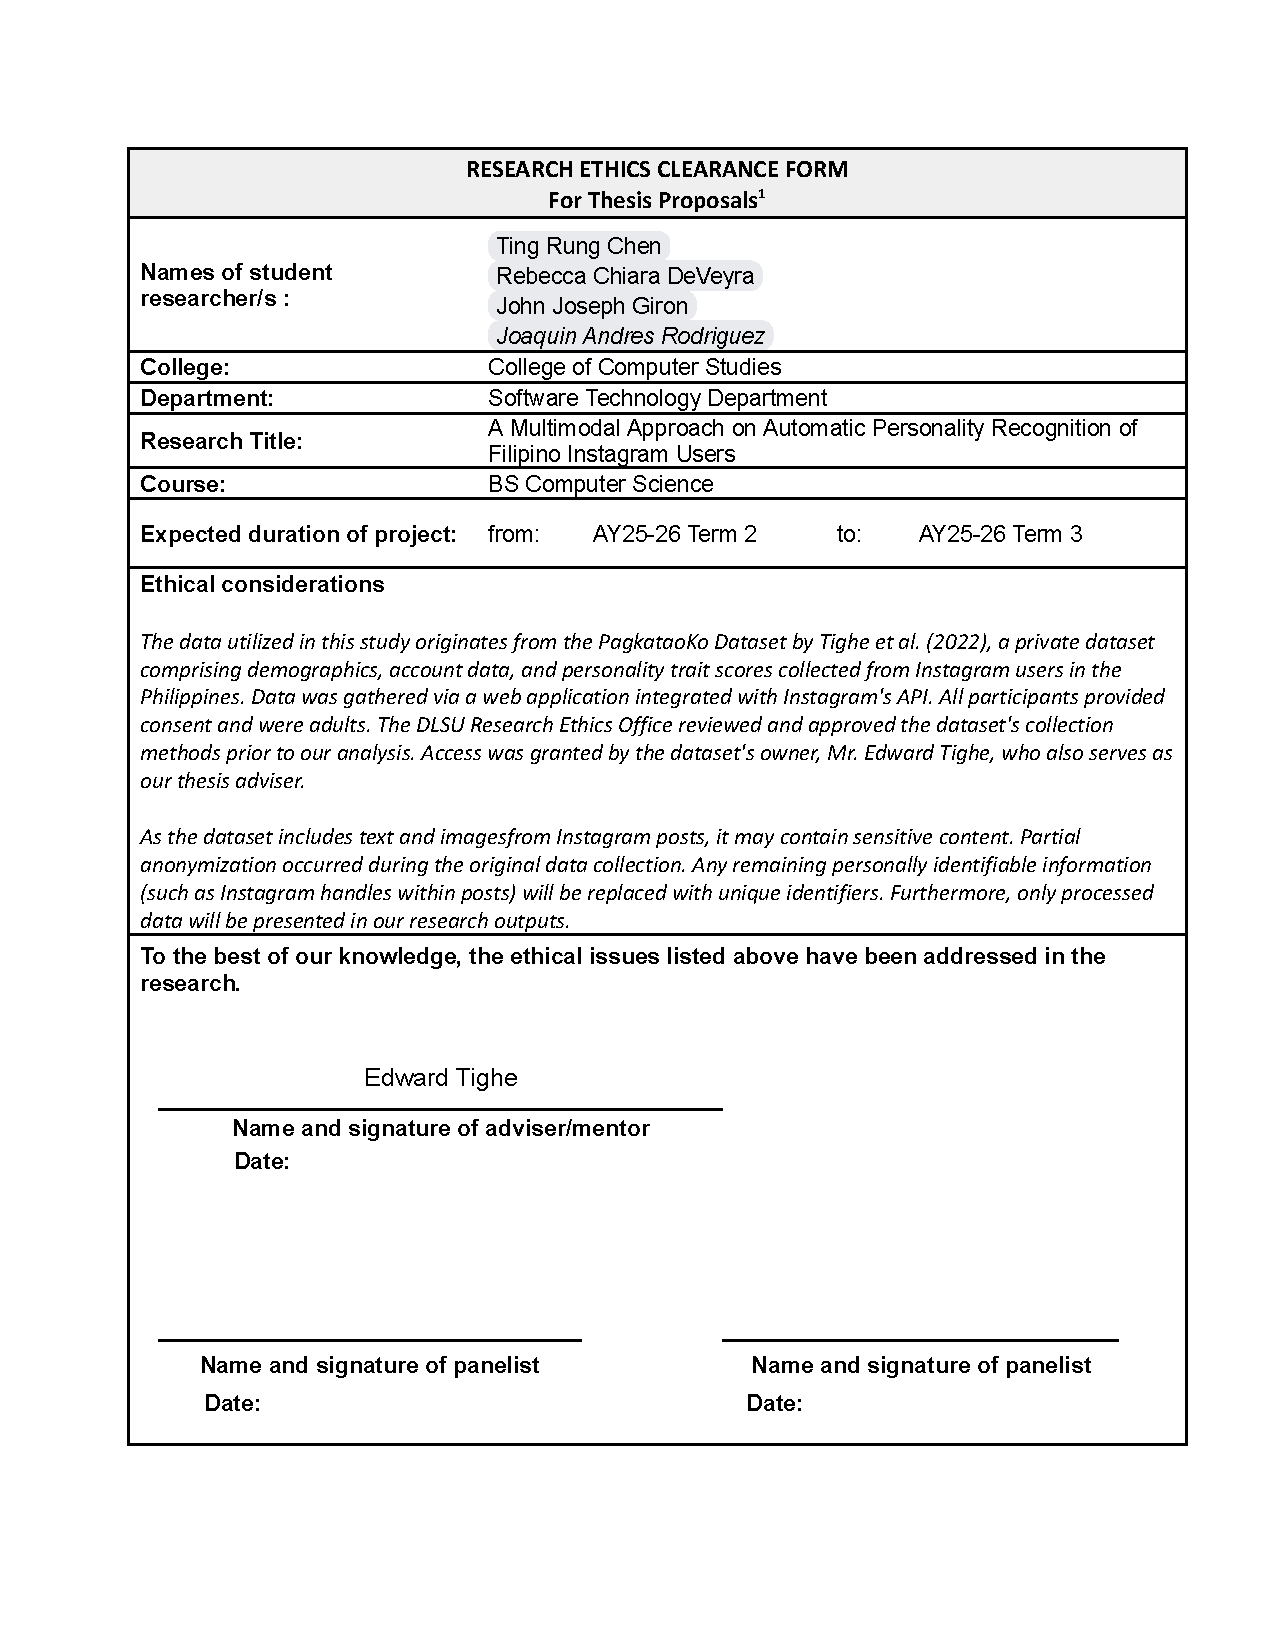
\includepdf[pages=-, scale = 0.9, pagecommand={}, offset = -30 0]{clearance.pdf}

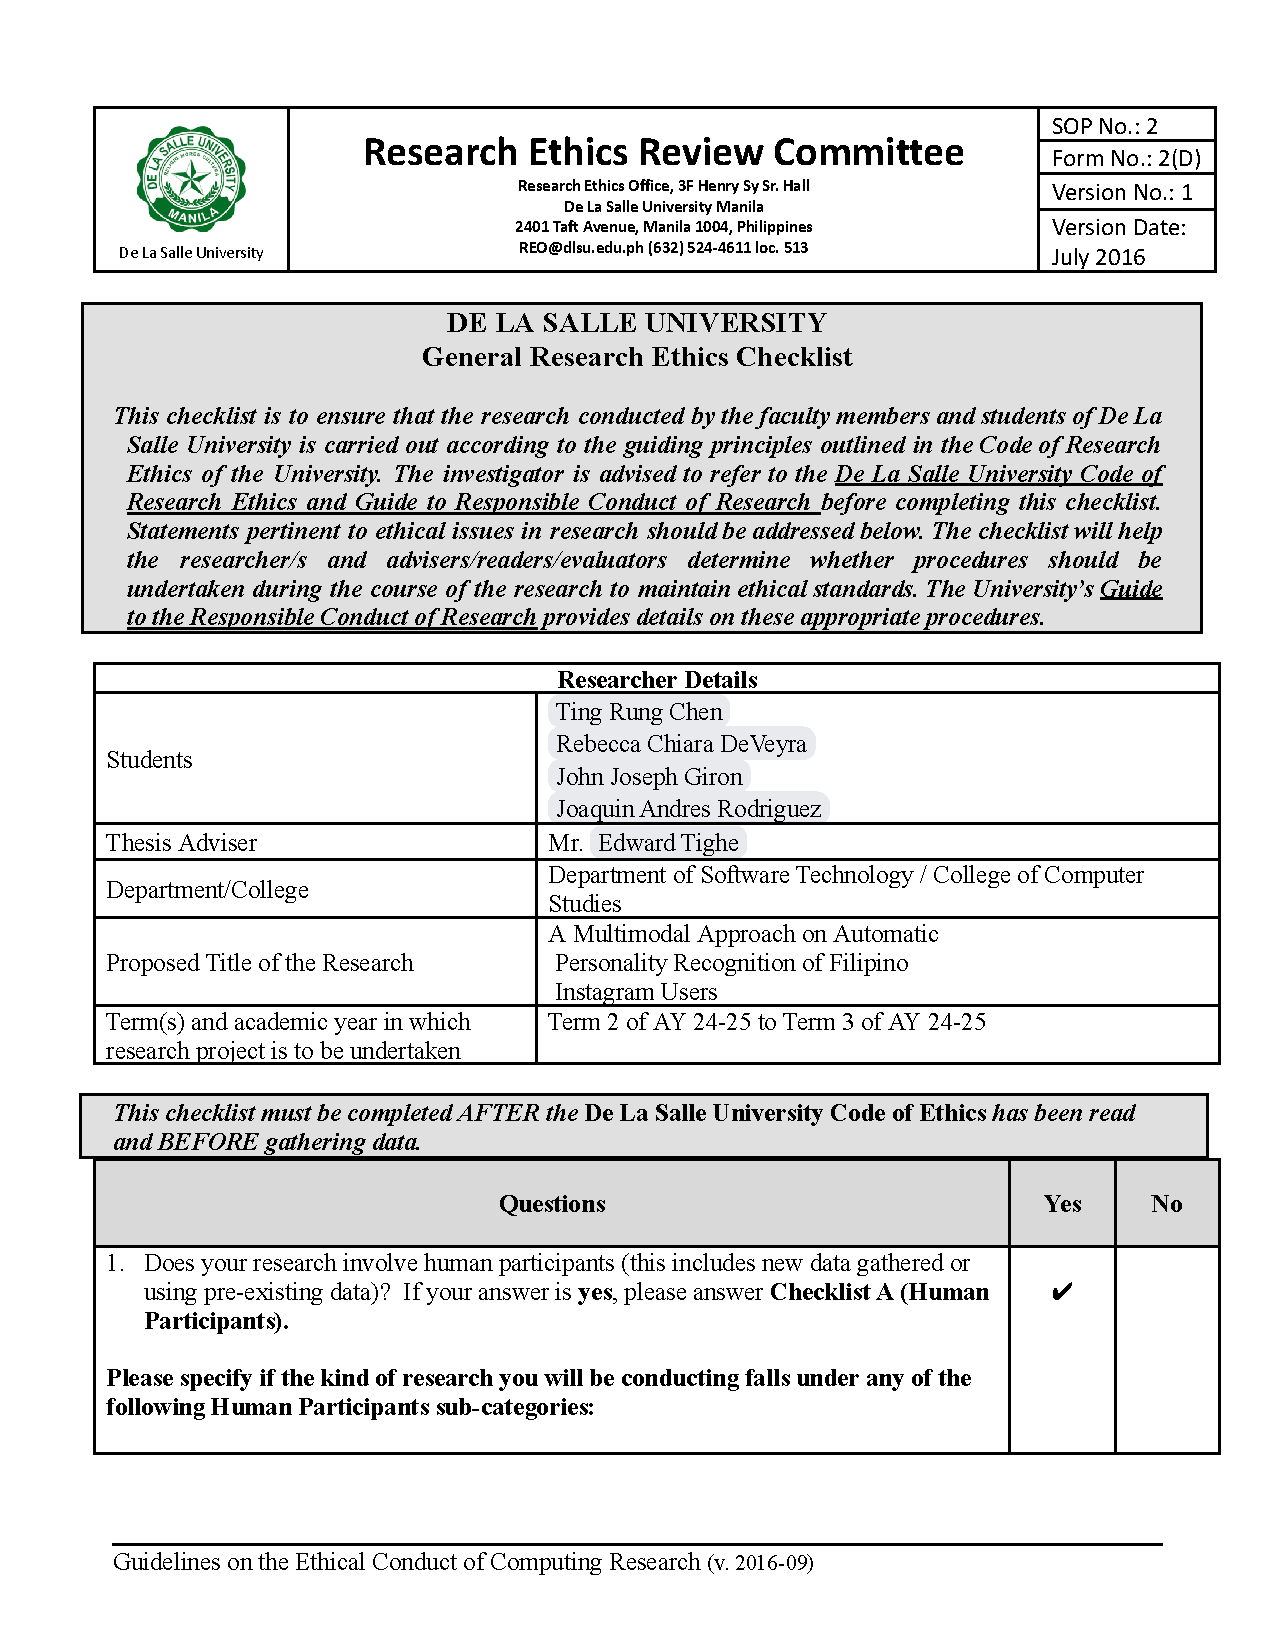
\includepdf[pages=-, scale = 0.9, pagecommand={}, offset = -30 0]{general_checklist.pdf}


\includepdf[pages=-, scale = 0.9, pagecommand={}, offset = -30 0]{checklist-A.pdf}

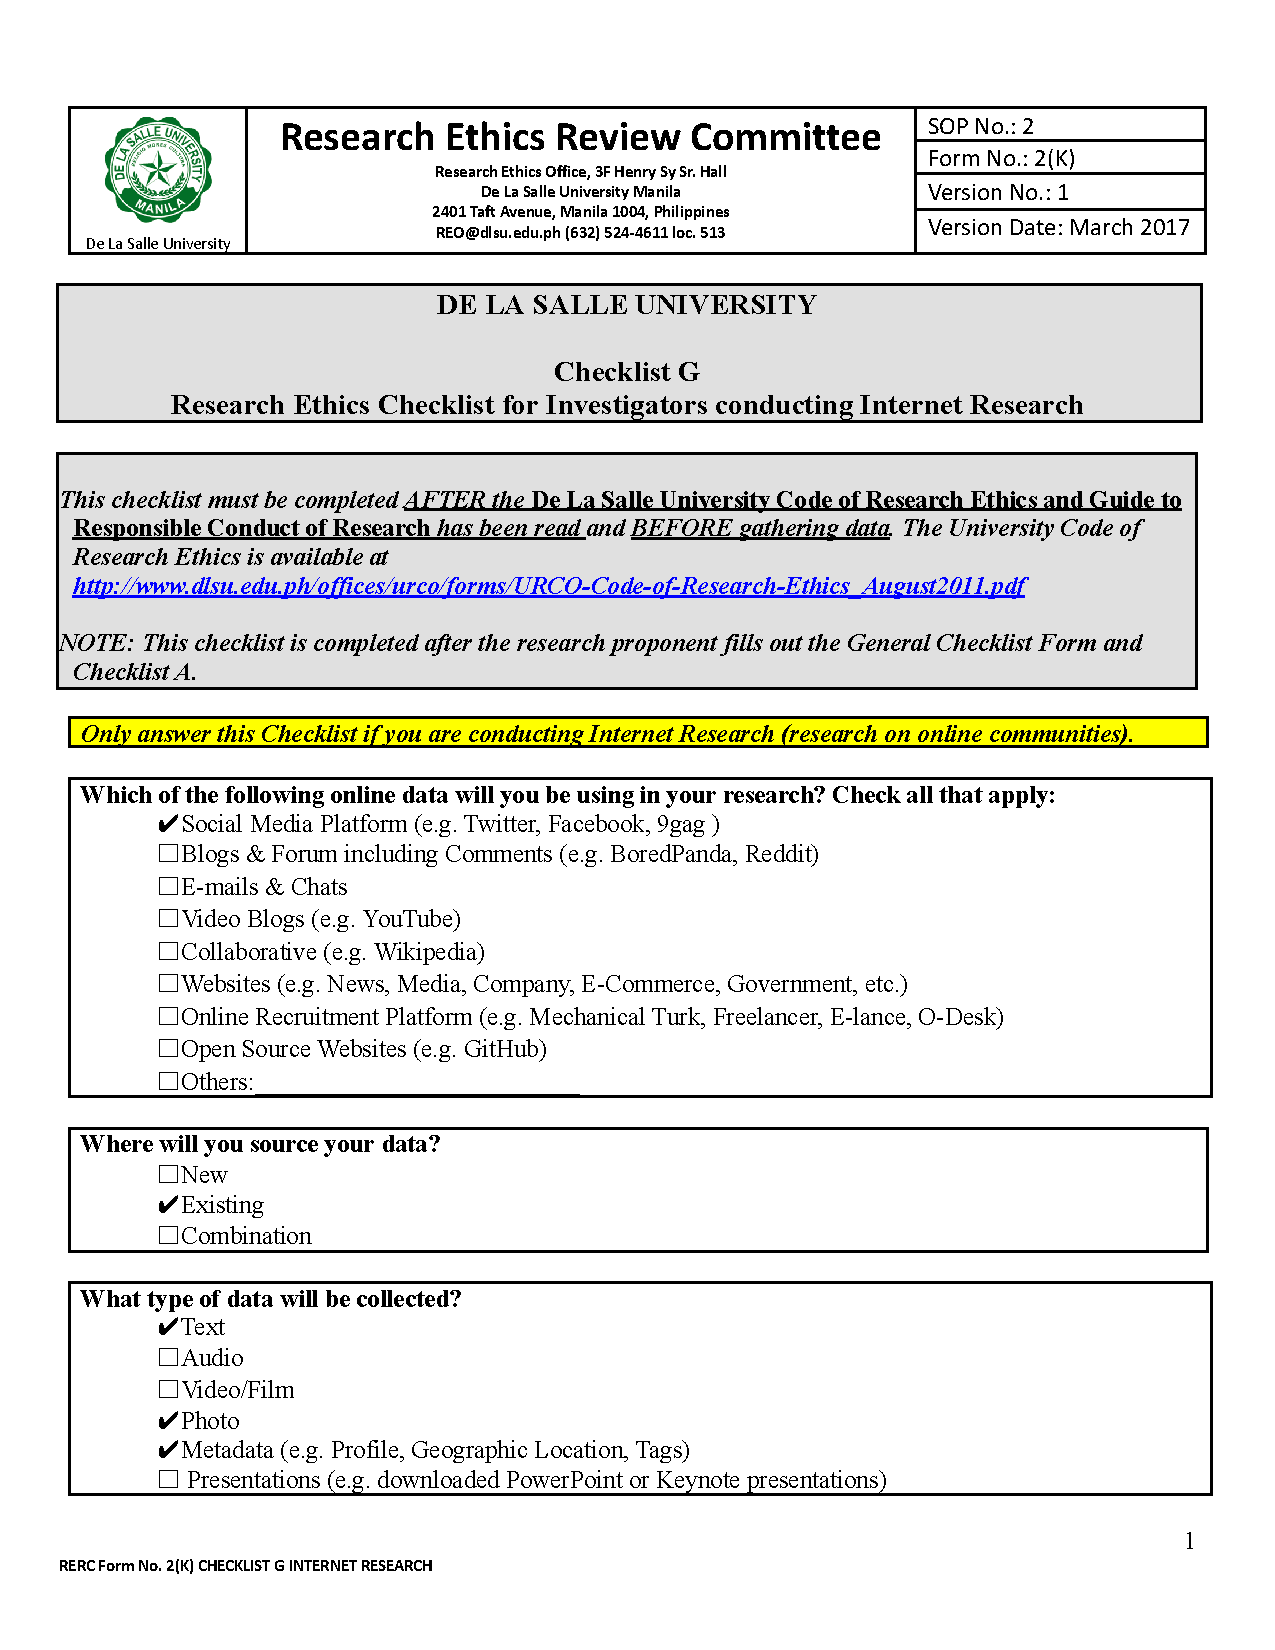
\includepdf[pages=-, scale = 0.9, pagecommand={}, offset = -30 0]{checklist-G.pdf}              %-- includes LaTeX source file for Appendix A
                                  %-- your job: **CREATE/EDIT** your own source file for the appendices
%\include{appendix_B}


\bibliographystyle{apacite}       %-- specified APA style for bibliograpy
                                  %-- more details about APA style citation can be found in www.ctan.org/tex-archive/biblio/bibtex/contrib/apacite/

                                  %-- bibliographic entries are handled via bibtex; refer to www.bibtex.org for more details


\bibliography{myreferences}       %-- the file "myreferences.bib" is a sample bibliography (bib) from SIGGRAPH 
                                  %-- your job: **CREATE/EDIT** your own bibliography file  

\end{document}

